%Copyright 2019 Christopher M. Jermaine (cmj4@rice.edu) and Risa B. Myers (rbm2@rice.edu)
%
%Licensed under the Apache License, Version 2.0 (the "License");
%you may not use this file except in compliance with the License.
%You may obtain a copy of the License at
%
%    https://www.apache.org/licenses/LICENSE-2.0
%
%Unless required by applicable law or agreed to in writing, software
%distributed under the License is distributed on an "AS IS" BASIS,
%WITHOUT WARRANTIES OR CONDITIONS OF ANY KIND, either express or implied.
%See the License for the specific language governing permissions and
%limitations under the License.
%===============================================================
\documentclass{article}

% General document formatting
\usepackage[margin=0.7in]{geometry}
\usepackage[parfill]{parskip}
\usepackage[utf8]{inputenc}
\usepackage{multirow}
\usepackage{xcolor,colortbl}
\usepackage{graphicx}
\usepackage{float}
% for copyright notice
\usepackage{textcomp}

\usepackage{listings}

\newenvironment{noindentitemize}
{ \begin{itemize}
 \setlength{\itemsep}{1.5ex}
  \setlength{\parsep}{0pt}   
  \setlength{\parskip}{0pt}
 \addtolength{\leftskip}{-2em}
 }
{ \end{itemize} }

\newenvironment{noindentitemize2}
{ \begin{itemize}
  \setlength{\itemsep}{0ex}
  \setlength{\parskip}{0pt}
  \setlength{\parsep}{0pt}   
  \addtolength{\leftskip}{-2em}  }
{ \end{itemize} }

\lstnewenvironment{SQL}
  {\lstset{
        aboveskip=5pt,
        belowskip=5pt,
        escapechar=!,
        mathescape=true,
        upquote=true,
        language=SQL,
        basicstyle=\linespread{0.94}\ttfamily\footnotesize,
        morekeywords={WHILE, DO, END},
        deletekeywords={VALUE, PRIOR},
        showstringspaces=true}
        \vspace{0pt}%
        \noindent\minipage{0.47\textwidth}}
  {\endminipage\vspace{0pt}}


% Related to math
\usepackage{amsmath,amssymb,amsfonts,amsthm}

\usepackage{fancyhdr}
\pagestyle{fancy}

% clear the default header and footer
\fancyhf{}
%\lfoot{\textcopyright Copyright Us}
\rfoot{\thepage}


\title{Tools \& Models for Data Science \\ Outliers Handout}
\date{}

% Set this length to 0pt if you don't want any lines!
\renewcommand{\headrulewidth}{0pt}

% Apply the fancy header style
\begin{document}
\maketitle
\thispagestyle{fancy}

\begin{SQL}
init min-priority queue $O$
for $x_1 \in X$:
  init max-priority queue $Q$
  for $x_2 \neq x_1 \in X$:
    insert $dist(x_1, x_2)$ into $Q$
    if $|Q| > k$
      remove max from $Q$
  insert $x_1$ into $O$ with key max$(Q)$
  if $|O| > m$
    remove point with min key from $O$

return $O$ 
\end{SQL}

\begin{figure}[H]
\begin{minipage}[T]{0.4\textwidth}
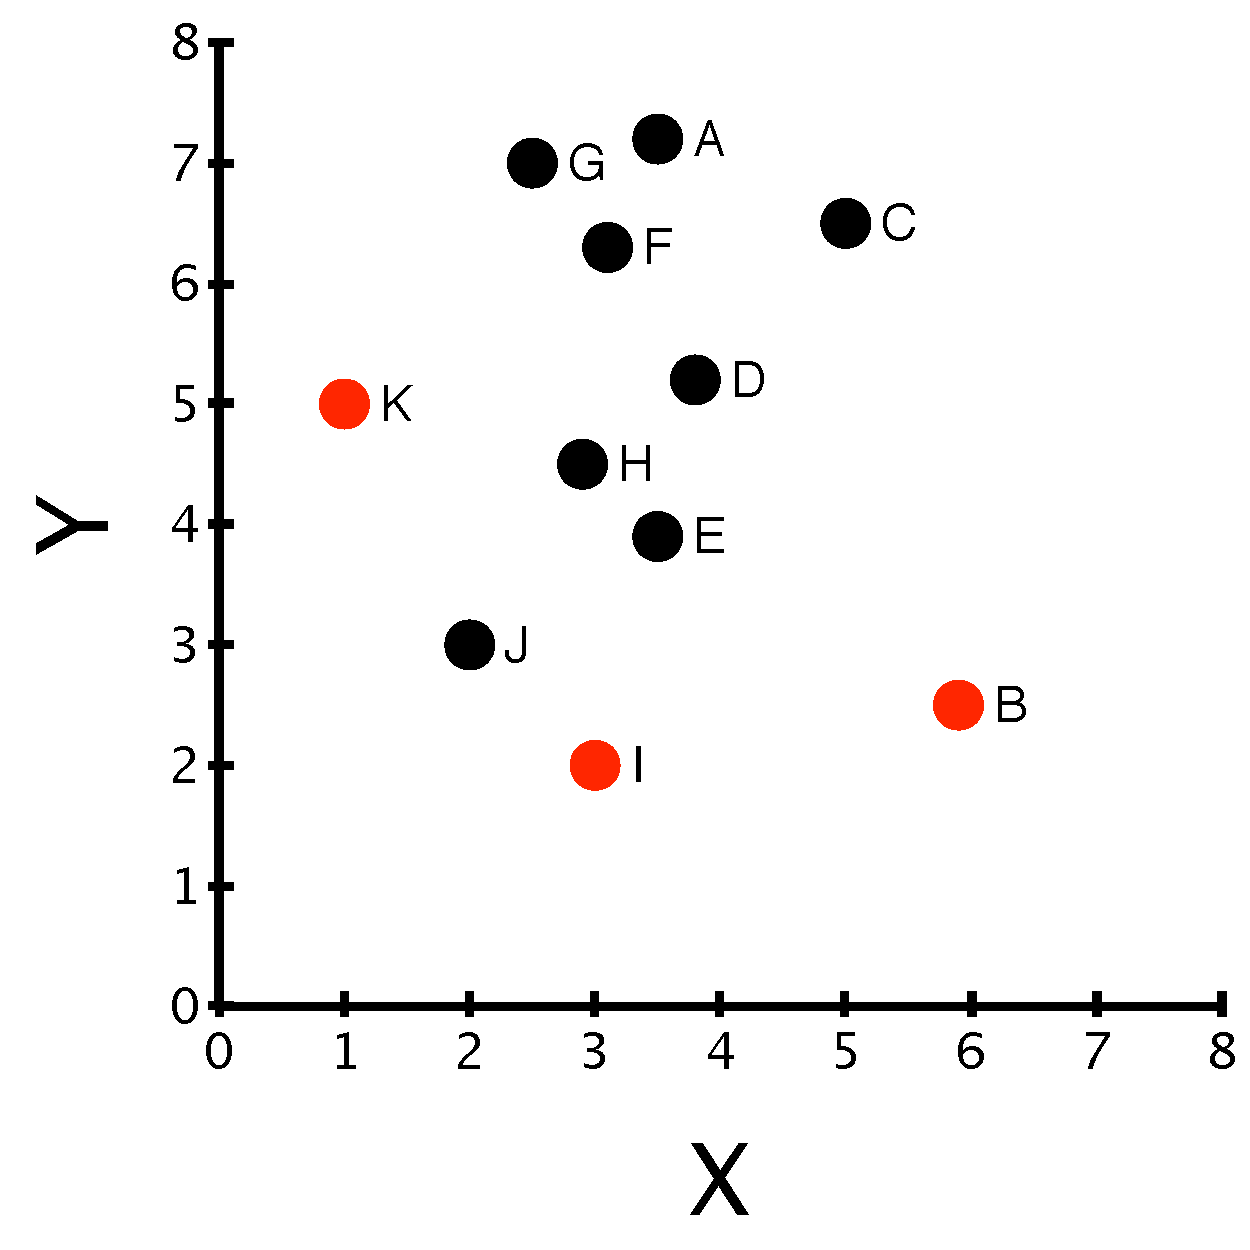
\includegraphics[width=1\textwidth]{lectOutliers/outliersPtsLabeled3Most.pdf}
\end{minipage}
%\end{figure}
\hspace{3em}
\begin{minipage}[T]{0.4\textwidth}

\begin {table}[H]
\begin{tabular}{|r|r|}
\hline
Point & 2NN distance \\ \hline
A & 1.02 \\ \hline
\textcolor{red}{B} & \textcolor{red}{2.94}  \\ \hline
C & 1.77 \\ \hline
D & 1.30 \\ \hline
E & 1.33  \\ \hline
F & 0.98 \\ \hline
G & 1.02 \\ \hline
H & 1.14 \\ \hline
\textcolor{red}{I} & \textcolor{red}{1.96} \\ \hline
J & 1.75 \\ \hline
\textcolor{red}{K} & \textcolor{red}{2.24} \\ \hline
\end{tabular}
\end{table}
\end{minipage}
\end{figure}

%}
%
%\end{minipage}
%


\begin{SQL}
O: { }
Pick a point: A
Q: { }
	Pick a point: B
	Q: {5.28}
	Q is not full

	Pick a point: C
	Q: {1.66, 5.28}
	Q is not full

	Pick a point: D
	Q: {1.66, 2.02, 5.28}
	Q is full
	Q: {1.66, 2.02}

	Pick a point: E
	Q: {1.66, 2.02, 3.30}
	Q is full
	Q: {1.66, 2.02}
	...
	Q: {0.98, 1.02}

O: {(1.02, A)}
O is not full

Next point: B
Q: { }
	Pick a point: A
	Q: {5.28}
	Q is not full

	Pick a point: C
	Q: {4.1, 5.28}
	Q is not full

	Pick a point: D
	Q: {1.77, 4.1, 5.28}
	Q is full
	Q: {1.77, 4.1}

	...

	Q: {2.78, 2.94}
O: {(1.02, A), (2.94, B)}

Finally, get
O: {(2.94, B), (2.24, K), (1.96, I)}

\end{SQL}

\end{document}